%================================================================================
%=============================== DOCUMENT SETUP =================================
%================================================================================

%\documentclass[lang=ngerman,inputenc=utf8,fontsize=10pt]{ldvarticle}
\documentclass[lang=ngerman,inputenc=utf8,fontsize=10pt]{ldvarticle}
%PACKAGES

\usepackage{parskip}
\usepackage{subfigure}
\usepackage{ifthen}
\usepackage{comment}
\usepackage{color}
\usepackage{colortbl}
\usepackage{soul}
\usepackage{tikz}
\usetikzlibrary{shapes,arrows}
\usepackage{tabularx}
\usepackage{lipsum}
\usepackage{pgfgantt}
\usepackage{amsmath}

\usepackage{color}

\usepackage[backend=biber,style=ieee,
doi=false,isbn=false,url=false,eprint=false]{biblatex}
\addbibresource{Relevant.bib}

\definecolor{lightgray}{rgb}{0.75,0.75,0.75}


\usepackage{tikz}
\usetikzlibrary{calc}
\usetikzlibrary{calendar}

\newcommand{\countweek}{\ifdate{equals=01-01}{\setcounter{weekcounter}{0}}{} \ifdate{Thursday}{\stepcounter{weekcounter}}{}}

% GanttHeader setups some parameters for the rest of the diagram
% #1 startdate
% #2 enddate
% #3 with of 
\def\GanttHeader#1#2#3{%
\newcounter{weeks}
\newcounter{weekcounter}
\def\withdes{3cm}
\def\hrows{0.4cm}
%get number of weeks
\calendar [dates=#1 to #2,day code={},
execute after day scope=
{\ifdate{Thursday}{\stepcounter{weeks}}{}}];

%get the currend KW
\calendar [dates=2021-01-01 to #1+-1,day code={},
execute after day scope=
{\countweek}];

%calcualate the shifts
\pgfmathsetmacro{\dayshift}{(\textwidth-\withdes)/(\theweeks*7)}

\tikzstyle{every day}=[anchor=mid]
\calendar [dates=#1 to #2,day code={},
execute after day scope=
{\countweek \ifdate{Thursday}{\node {\tiny\textbf{\theweekcounter}};}{} 
	\ifdate{Sunday}{\draw[thick] (0,-0.5*\hrows) -- +(0,\hrows);}{} 
	\ifdate{day of month=15}{\node[] at (0,\hrows) {\small{\tikzmonthtext}};}{} 
	\ifdate{day of month=1}{\draw[thick] (0,0.5*\hrows) -- +(0,\hrows);}{}
	\pgftransformxshift{\dayshift}}] 
at (\withdes,0); %set position

%setup descriptions
\draw[very thick] (0,0.5*\hrows) rectangle +(\withdes, \hrows);
\draw[very thick] (0,-0.5*\hrows) rectangle +(\withdes, \hrows);
\draw[very thick] (\withdes,0.5*\hrows) rectangle +(\textwidth-\withdes, \hrows);
\draw[very thick] (\withdes,-0.5*\hrows) rectangle +(\textwidth-\withdes, \hrows);
\node[] at (0.5*\withdes,\hrows) {\small{\textbf{Month}}};
\node[] at (0.5*\withdes,0) {\small{\textbf{Week}}};
}


% This macro adds a task to the diagram
% #1 Row of the Task
% #2 Task's name
% #3 Starting Week
% #4 Duration (Weeks)
\def\Task#1#2#3#4{%
\begin{scope}[shift={(0,-0.2*\hrows-#1*\hrows)}]
  \filldraw[fill=black!20,thick] (0,-0.5*\hrows) rectangle +(\textwidth, \hrows);
\node[anchor=west] at (1mm,0) {\small{\textbf{#2}}};
 \filldraw[color=red] (\dayshift*7*#3+\withdes,-0.45*\hrows) rectangle +(\dayshift*7*#4+0cm,0.9*\hrows);
  \foreach \x in {0,...,\theweeks} {
    \draw[thick] (\dayshift*7*\x+\withdes,-0.5*\hrows) -- +(0,\hrows);
}
\end{scope}
}







\usetikzlibrary{matrix}


\DeclareMathOperator{\vect}{vec}
\DeclareMathOperator{\rank}{rank}

%================================================================================
%================================= TITLE PAGE ===================================
%================================================================================

\title{Combining Matrix Representations for Structured Approximation of Neural Network Weight Matrices}
\subtitle{Projectplan}
\author{Stepahn Nüßlein}

\date{\today}

\begin{document}


	\maketitle
	\thispagestyle{empty}
	\vspace*{2cm}
	\hrule

\section*{Motivation}

As the matrices for fully connected layers get larger the evaluation of the neural nets get computationally more expensive. This is often problematic as the computational resources are a limiting factor, especially on embedded or mobile systems.
Therefore different matrix representations to reduce the computational cost are being explored.

A possible representation are sequentially semiseperable matrices. These have a certain underlying structure.
The structure of the sequentially semiseperabel matrix is often determined by a underlying physical system or the construction of the matrix.
The matrices in neural networks do not necessarily have the same underlying structure.
Even if the matrix is close to a sequentially semiseperable matrix the structural parameters might not be know.
To increase the number of matrices that can be represented we also allow combinations of sequentially semiseperable matrices.

To represent the matrices, possible algorithms to derive the representation are investigated and tested.
%To represent the matrices, an algorithm to derive the representation is needed.
	%\item Both approxiamtion of Matrix in some Norm ($\|\|_F$,$\|\|_1$,$\|\|_\infty$ or similar) also Accuracy on Data set




\vspace*{1cm}
\hrule

\newpage

\section{Project Description}

\subsection*{Goals}

\begin{itemize}

	\item\textbf{Matrix approximation with reduced cost} Find a matrix approximation. This requires a formal definition, as well as a reference implementation.
	\item\textbf{Algorithm to construct said approximation} Development of an algorithm to calculate the approximation. Also implement a reference implementation
	\item\textbf{Theoretical description} Compile the theoretical properties that can be derived.
	\item\textbf{Evaluate approximation in practical examples} Evaluate the performance on weight matrices from pretrained models form Pytorch. This includes the behavior of the approximation algorithm, the computational cost as well as the performance of the neural net
\end{itemize}





\subsection*{Approach}

These assumptions and properties are underlying the idea:
\begin{itemize}
	\item Matrices in fully connected layers often have full rank. This means that a rank reduction is not easily possible (with some caveats, as it is not certain that this is the relevant ingredient) \cite{martin_implicit_2018}
	\item To get the optimal trade of between accuracy and cost it should be possible to adapt the accuracy of the approximation by changing hyper parameters of the approximation.
\end{itemize}

State-Space representation have many hyperparameters like input and output dimensions, these have to be chosen. By setting the input and output dimensions we fix an segmentation of the representable matrices.

The matrices in a neural net might not have an underlying structure that can be represented.
Therefore it might be interesting if the matrices in an neural net can be better described with combinations of different representations.
This might be the sum of state-space representations. These might have the same or different input and output dimensions.
It might be also interesting to use permutations of the input and output to obtain segments with low rank.
A similar representation with products of SSS Representations with non matching output and input dimensions might also be possible, but is harder to describe.

\subsubsection*{Segmentation}
One prerequisite is finding appropriate segmentation of the Matrix. This either includes finding a existing way of finding a segmentation and implementing it.
Or coming up with a an algorithm to segment a matrix.

\subsubsection*{Computational cost}
The computational cost of evaluation a matrix vector product is related to the number of parameters.
For the state space representation the number of multiplications is equal to the number of entries in the $A$,$B$,$C$ and $D$ matrices. These depend on the dimensions of the input and output and on the number of states.

\subsubsection*{Properties}
The properties of the representations should be tested in terms of computational cost, storage requirements and performance in neural nets.
The computational stability of the resulting algorithm might be tested numerically. This might be for further interest if the evaluation is done on an 32-bit architecture.

\section*{Some Results}
In the following some results are summed up:

\subsection*{Addition of Systems}
One idea was that the sum of two systems with different input and output dimensions might be able to represent a wider class of matrices.
It is questionable that this class is far bigger as the relation 
\begin{equation}
	\rank(A) \leq \rank(H_a) + \rank(H_b) 
\end{equation}
holds true for all submatrices that do not contain $D$-matrices.
There might be some benefits in the close vicinity to the diagonal but it is unclear if this is relevant.

A possible idea would be decomposing a system in two parallel systems.
This could be done by state transforms. But it is unclear if state transformations that lead to the needed zeros in $A$.


\subsection*{Changes to size of the input and output dimensions}
I already programmed code to change the size of the inputs and outputs. The code also preserves minimality.
In some cases this results in a increasing/decreasing state dimensions. This depends on the parts of $D$ that are included or excluded. 
This does not depend on the rest of the matrix (Similar to the shift invariance principle).
This might be different for cases where an later approximation is done.

\section{Some Questions that came up}

\subsection*{Approximation}
An approximation of an system can be done using the hankel rank approximation. 
How does this relate to the matrix approximations for different norms and use cases?
%If the implementation is balanced and the states are ordered with respect to the according $\sigma$s the state dimension can be reduced by simply dropping columns and rows from the matrices.

\subsection*{Importance of $D$}
As there is no restriction of the $D$-Matrix, it is quite versatile.
Is it possible to permute rows and columns in a way that makes use of this property?

\section{Further Ideas:}

\subsection*{Segmentation of Matrix}
Derive an first informed guess on the segmentation based on a model of the expected hankelrank. This might first include a model with constant input and output dimensions. 
%Maybe later different dimenstions
After this move boundaries if this gives an computational advantage.

\subsection*{Derive Permutations}
Use algorithm from \cite{ulfarsson_sparse_2015} or different algorithm to get a sparse + low rank representation.
Then group the sparse elements and move them into the $D$ matrices.
This also results in a segmentation.
And then represent the permuted matrix using a system. 


%\subsubsection*{Calculation of Representation}
%There are two possible ideas to get the wanted representation:
%
%\paragraph{Optimization Problem}
%Convert the given properties into manifolds and objective functions and use optimization techniques.
%This might be easier to define, but will possibly result in a problem with a very high number of dimensions. Maybe it is possible to express it as some standard problem, then it would be possible to use standard solvers and use existing guarantees and runtime estimates.
%
%\paragraph{Iterative Methods}
%Use an approach similar to Matching pursuit. Here the dictionary $D$ would be a subset of all Sequentially Semiseperable Matrices. This requires some description of a qasi-inner-product and an way to find an approximation of the closest element in $D$.
%As $D$ will have infinitely many dimensions, this might be quite involved.



\section{Workpackages}

\begin{itemize}
	\item \textbf{Literature review:}
	\begin{itemize}
			\item \textbf{Existing Decompositions:} Low Rank+Sparse, Multiscale Low rank \cite{chandrasekaran_sparse_2009,ong_beyond_2016,yu_compressing_2017}
			\item \textbf{Sparsity:} Appropriate Sparsity Measures \cite{ulfarsson_sparse_2015,parekh_improved_2017}
			\item \textbf{Existing Algorithms:} Look into the structure of related algorithms
		\end{itemize}
	\item \textbf{Evaluation:} 
		\begin{itemize}
			\item \textbf{Selection:} Choose appropriate assumptions
			\item \textbf{Theoretical considerations:} Try the theoretical questions outlined above.
		\end{itemize}
	\item \textbf{Implementation:} 
		\begin{itemize}
			\item \textbf{Implement Algorithm(s):} Based on previous exploration implement tests and algorithms to construct the representation.
			\item \textbf{Generate Tests:} Generate testdata and pipeline to test them, including meta-analysis (speed of convergence...)
		\end{itemize}
	\item \textbf{Analysis:} 
		\begin{itemize}
			\item \textbf{Setup Test}
			\item \textbf{Evaluation I:} Evaluation on tailor-made examples: Combination of Sequentially Semiseperable Matricies %(I think we need more than $\min(n,m)$ rank sub matrices until the standard SVD not be able to recover the structure?, but even then it might be interesting, as we can reduce the computations)
			\item \textbf{Evaluation II:} Random matrices with different parameters
			\item \textbf{Evaluation III:} Evaluation on AI matrices
		\end{itemize}
	\item \textbf{Evaluation and discussion:} 
		\begin{itemize}
			\item \textbf{Revisiting the theory:} Explanations for experienced behavior?
			\item \textbf{Description of performance:} Describe the tests and visualize the results.
			\item \textbf{Discussion:} Evaluate the results and put it into context.
		\end{itemize}
	\item \textbf{Presentation of results:} Write down the research and compile it to a thesis. 
\end{itemize}

\section{Time Table}



	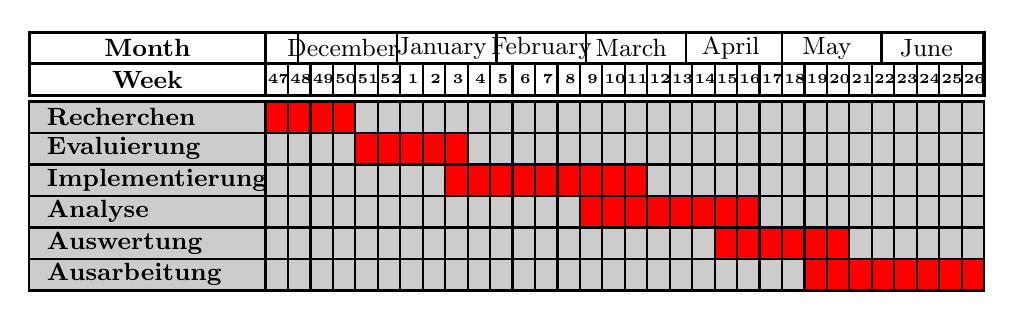
\begin{tikzpicture}
	\GanttHeader{2021-11-21}{2022-06-30}{\textwidth}


	\Task{1}{Recherchen}{0}{4}
	\Task{2}{Evaluierung}{4}{5}
	\Task{3}{Implementierung}{8}{9}
	\Task{4}{Analyse}{14}{8}
	\Task{5}{Auswertung}{20}{6}
	\Task{6}{Ausarbeitung}{24}{8}
	\end{tikzpicture}






\section{Risk Analysis}

Computation effort might not be lower than the effort for regular matrix vector product.
\newline\textbf{Likelihood:} Risk is hard to determine upfront as it depends on how many fast the approximation converges.
\newline\textbf{Mitigation:} Test practical examples at an early stage of the thesis and.

Unable to find an appropriate algorithm
\newline\textbf{Likelihood:} Quite likely as it is a very underdetermined problem with many parameters
\newline\textbf{Mitigation:} use more computation-time, reduction of degrees of freedom by requiring some artificial condition (e.g. set the structure of the submatrices)


\printbibliography

\end{document}
